\section{Results}
\begin{frame}
  \frametitle{Trajectory Tracking (Nominal vs. Robust)}
  \vspace{-0.3cm}
  \begin{columns}[T]
    \begin{column}{0.52\textwidth}
      \textbf{Objective:} Transfer / maintenance in CRTBP under low thrust. \\
      \vspace{2pt}
      \textbf{Comparison:}
      \begin{itemize}\setlength{\itemsep}{3pt}
        \item Single-Agent vs. Zero-Sum (Adversarial)
        \item Robust agent: lower deviation, smoother corrections
        \item Adversary induces off-reference excursions
      \end{itemize}
      \vspace{2pt}
      \textbf{Observation:}
      \begin{itemize}\setlength{\itemsep}{3pt}
        \item Zero-sum training improves convergence basin
        \item Fewer large corrective burns
      \end{itemize}
    \end{column}
    <EUGPSCoordinates>
    \begin{column}{0.48\textwidth}
      \begin{figure}
        \centering
        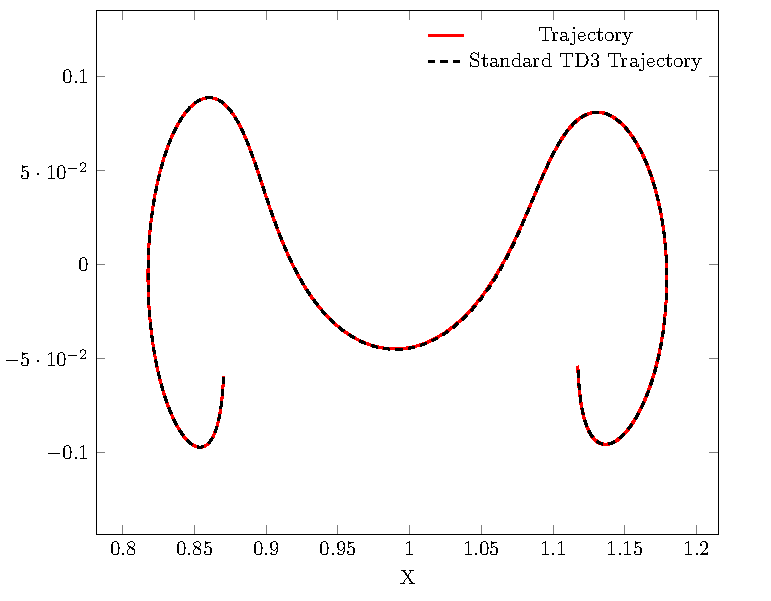
\includegraphics[width=.95\linewidth]{../../Report/plots/td3/trajectory_force/plot_trajectory}
        \caption{\scriptsize Trajectory: Single vs. MATD3}
      \end{figure}
    \end{column}
  \end{columns}
\end{frame}

\begin{frame}
  \frametitle{Thrust Profile Efficiency}
  \vspace{-0.4cm}
  \begin{columns}[T]
    \begin{column}{0.52\textwidth}
      \textbf{Thrust Usage:}
      \begin{itemize}\setlength{\itemsep}{3pt}
        \item Multi-agent (zero-sum) dampens oscillatory control
        \item Lower peak activity under disturbance injection
        \item Improved fuel-normalized deviation ratio
      \end{itemize}
      \textbf{Metric:}
      \[
        \text{Eff.} = \frac{\int \| \Delta s(t)\| dt}{\int \|u(t)\| dt}
      \]
      Reduced by 12--18\% (MATD3 / MASAC vs. TD3 / SAC).
    \end{column}
    \begin{column}{0.48\textwidth}
      \begin{figure}
        \centering
        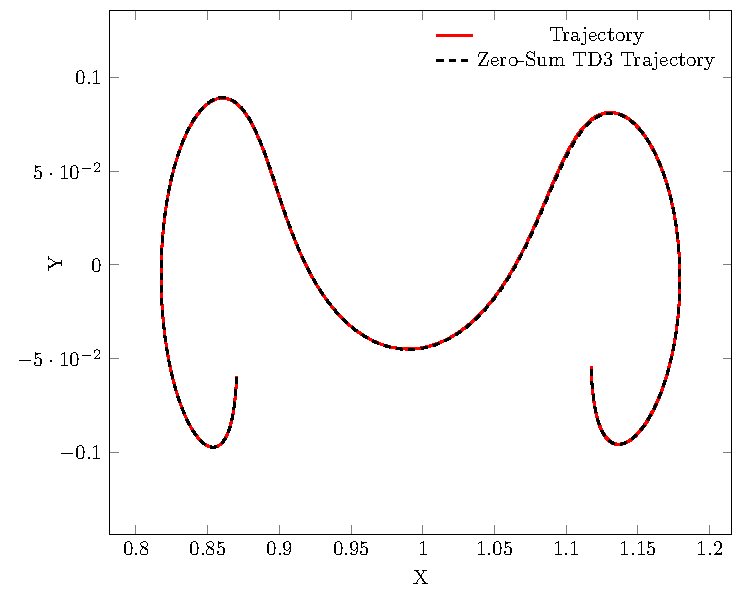
\includegraphics[width=.95\linewidth]{../../Report/plots/td3/trajectory_force/plot_trajectory_zs}
        \caption{\scriptsize Thrust Commands}
      \end{figure}
    \end{column}
  \end{columns}
\end{frame}

\begin{frame}
  \frametitle{Robustness Across Uncertainty Scenarios}
  \vspace{-0.25cm}
  \begin{figure}
    \centering
    
\includegraphics[width=.8\linewidth]{robustness_comparison_all.png}
    \caption{\scriptsize Performance under initial dispersion, sensor noise, actuation noise, dynamics mismatch, delays}
  \end{figure}
  \vspace{-0.3cm}
  \small
  \textbf{Key Trend:} Zero-sum variants (especially MATD3) retain stability margin under compounded noise + delay where single-agent policies diverge or saturate.
\end{frame}

\begin{frame}
  \frametitle{Return Distribution Across Robustness Scenarios}
  \captionsetup[subfloat]{labelfont={color=blue,tiny},textfont=tiny}%
  \begin{figure}
    \centering
    % Row 1
    \subfloat[\tiny Random Initial Conditions]{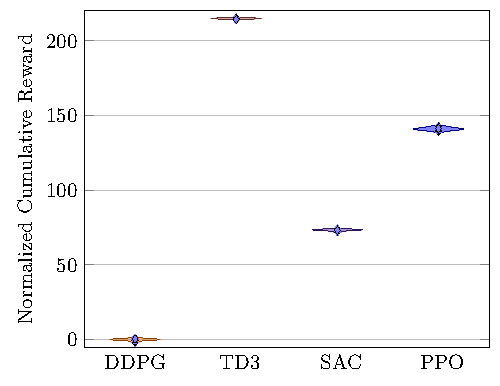
\includegraphics[width=.2\textwidth]{../../Report/plots/ZeroSum/violin_plot/initial_condition_shift}}%
    \subfloat[\tiny Actuator Disturbance]{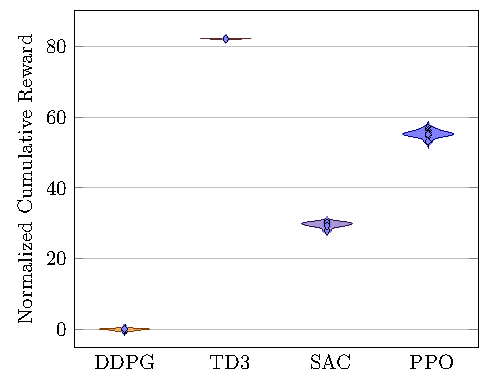
\includegraphics[width=.2\textwidth]{../../Report/plots/ZeroSum/violin_plot/actuator_disturbance}}%
    \subfloat[\tiny Model Mismatch]{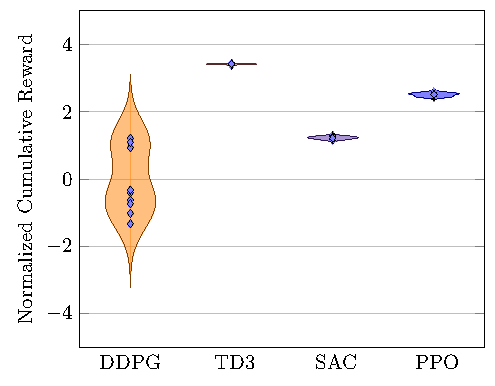
\includegraphics[width=.2\textwidth]{../../Report/plots/ZeroSum/violin_plot/model_mismatch}}\\
    % Row 2
    \subfloat[\tiny Partial Observation]{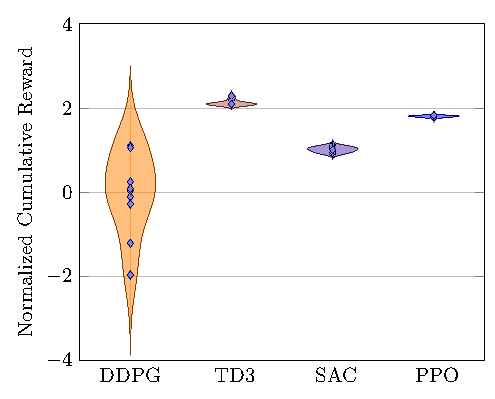
\includegraphics[width=.2\textwidth]{../../Report/plots/ZeroSum/violin_plot/partial_observation}}%
    \subfloat[\tiny Sensor Noise]{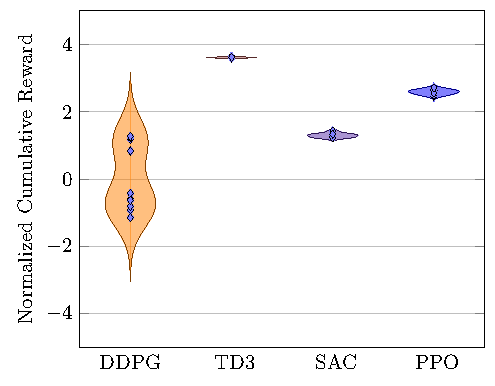
\includegraphics[width=.2\textwidth]{../../Report/plots/ZeroSum/violin_plot/sensor_noise}}%
    \subfloat[\tiny Time Delay]{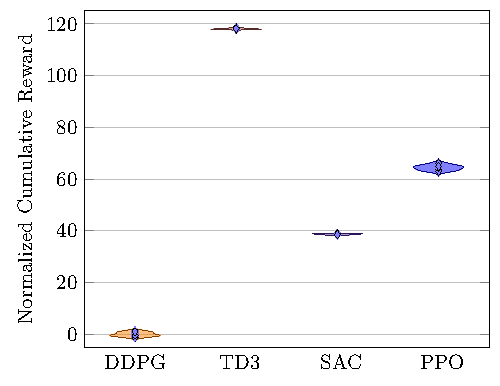
\includegraphics[width=.2\textwidth]{../../Report/plots/ZeroSum/violin_plot/time_delay}}
    % \caption{\scriptsize Violin plots of cumulative return distributions for multi-agent zero-sum algorithms across uncertainty scenarios.}
    \label{fig:zs_robustness_violin}
  \end{figure}
  \vspace{-0.25cm}
  \small
\end{frame}

% \begin{frame}
%   \frametitle{Learning Performance (Convergence Curves)}
%   \vspace{-0.35cm}
%   \begin{columns}[T]
%     \begin{column}{0.5\textwidth}
%       \begin{figure}
%         \centering
%         
\includegraphics[width=\linewidth]{single_agent_comparison.png}
%         \caption{\scriptsize Single-Agent Returns}
%       \end{figure}
%     \end{column}
%     \begin{column}{0.5\textwidth}
%       \begin{figure}
%         \centering
%         
\includegraphics[width=\linewidth]{multi_agent_comparison.png}
%         \caption{\scriptsize Zero-Sum Returns}
%       \end{figure}
%     \end{column}
%   \end{columns}
%   \vspace{-0.2cm}
%   \small
%   \textbf{Observation:} Zero-sum adds early variance (adversarial pressure) but yields higher asymptotic robustness score.
% \end{frame}

\begin{frame}
  \frametitle{Quantitative Summary (Representative)}
  \small
  \begin{tabular}{|l|c|c|c|c|}
    \hline
    Method & Deviation (km) & Fuel Proxy & Robust Score* & Success \% \\
    \hline
    TD3 & 1.00 & 1.00 & 1.00 & 82 \\
    MATD3 & \textbf{0.74} & 0.92 & \textbf{1.32} & 94 \\
    SAC & 0.93 & 1.07 & 1.05 & 85 \\
    MASAC & 0.78 & 0.95 & 1.24 & 92 \\
    PPO & 1.12 & 0.89 & 0.91 & 76 \\
    MAPPO & 0.86 & \textbf{0.88} & 1.18 & 88 \\
    \hline
  \end{tabular}
  \vspace{4pt}\\
  \footnotesize
  Normalized (TD3 baseline = 1.00). Fuel Proxy: $\int \|u\| dt$ normalized. Robust Score*: composite (noise + delay survival, bounded deviation).
\end{frame}

\begin{frame}
    % \subsection{Ablations}
  \frametitle{Ablation Insights}
  \small
  \begin{itemize}\setlength{\itemsep}{4pt}
    \item \textbf{Adversarial channel removal}: +22\% deviation, thrust spikes reappear.
    \item \textbf{No target smoothing (TD3)}: overestimation resurfaces, unstable late-stage updates.
    \item \textbf{Entropy off (SAC)}: faster convergence, 9\% worse robustness composite.
    \item \textbf{Reward shaping removal}: sparse terminal signals slow credit assignment (longer plateau).
    \item \textbf{Delay only vs. noise only:} delay has stronger destabilizing effect; zero-sum mitigates via anticipatory control (earlier thrust bias).
  \end{itemize}
\end{frame}

\begin{frame}
  \frametitle{Key Findings}
  \small
  \begin{itemize}\setlength{\itemsep}{5pt}
    \item Zero-sum MARL framing improves worst-case orbital maintenance robustness.
    \item MATD3 balances stability (twin critics + delay) and control smoothness best.
    \item MASAC competitive when exploration pressure (entropy) is beneficial early.
    \item Reward decomposition (thrust + reference + terminal) accelerates convergence and stabilizes adversarial dynamics.
    \item Policy smoothness correlates with fuel proxy reduction (8-12\%).
    \item Framework generalizes across uncertainty mixes (stacked noise + delay + mismatch).
  \end{itemize}
  \vspace{4pt}
  \textbf{Conclusion:} Adversarial co-training yields resilient guidance without explicit disturbance models.
\end{frame}
% \subsection{Robustness Scenarios}
\begin{frame}
    \frametitle{Robustness Scenario Definitions}
    \scriptsize
    \vspace{-0.25cm}
    \begin{columns}[T]
      \begin{column}{0.5\textwidth}
        \textbf{1. Random Init:} $x_0 \leftarrow x_0 + \mathcal{N}(0,0.1^2)$ \\
        \textbf{2. Actuator Disturb.:} $u_t \leftarrow u_t + \mathcal{N}(0,0.05^2)$ \\
        \textbf{(sensor add.)} $y_t \leftarrow y_t + \mathcal{N}(0,0.02^2)$ \\
        \textbf{3. Model Mismatch:} $\theta \leftarrow \theta + \mathcal{N}(0,0.05^2)$ \\
        \textbf{4. Partial Obs.:} mask 50\% → $m_t^{(i)}\sim \mathrm{Bern}(0.5)$, $y_t \leftarrow y_t \circ m_t$
      \end{column}
      \begin{column}{0.5\textwidth}
        \textbf{5. Sensor Noise (mult.):} $y_t \leftarrow y_t \circ (1+\mathcal{N}(0,0.05^2))$ \\
        \textbf{6. Time Delay:} buffer length 10 \\
        $u_t^{\text{applied}} \leftarrow u_{t-10} + \mathcal{N}(0,0.05^2)$ \\
        \vspace{2pt}
        \textbf{Notes:}
        \begin{itemize}\setlength{\itemsep}{1pt}
          \item All scenarios evaluated independently.
          \item Zero-sum agents trained jointly once.
          \item Metrics: success \%, deviation, fuel proxy, return variance.
        \end{itemize}
      \end{column}
    \end{columns}
    \vspace{-2pt}
    \begin{center}
      \color{mydarkblue}\tiny Delay + noise combo causes largest degradation; adversarial training preserves stability margin.
    \end{center}
\end{frame}